\documentclass[tikz,border=7pt]{standalone}

\usepackage{iftex}
\ifPDFTeX
  \PackageError{matrix-figure}{This figure requires XeTeX or Tectonic}{Compile with xelatex or tectonic.}
\fi
\usepackage{fontspec}
\usepackage{xeCJK}
\usepackage{amsmath}
\usepackage{unicode-math}
\usepackage{xcolor}
\usepackage{tikz}
\usetikzlibrary{arrows.meta,positioning}

\providecommand{\FigureUseLocalFonts}{0}
\ifnum\FigureUseLocalFonts=1
  \setmainfont{NotoSansCJKtc-Regular.otf}[Path=\FigureSansFontPath]
  \setsansfont{NotoSansCJKtc-Regular.otf}[Path=\FigureSansFontPath,BoldFont=NotoSansCJKtc-Bold.otf]
  \setCJKmainfont{NotoSansCJKtc-Regular.otf}[Path=\FigureSansFontPath]
  \setCJKsansfont{NotoSansCJKtc-Regular.otf}[Path=\FigureSansFontPath,BoldFont=NotoSansCJKtc-Bold.otf]
  \setmathfont{STIXTwoMath.otf}[Path=\FigureMathFontPath]
\else
  \setmainfont{Noto Sans CJK TC}
  \setsansfont{Noto Sans CJK TC}
  \setCJKmainfont{Noto Sans CJK TC}
  \setCJKsansfont{Noto Sans CJK TC}
  \setmathfont{STIX Two Math}
\fi

\definecolor{FigureInk}{HTML}{253142}
\definecolor{FigureGrid}{gray}{0.78}
\definecolor{FigureCurve}{gray}{0.18}
\definecolor{FigurePoint}{gray}{0.42}
\definecolor{PanelFill}{gray}{0.94}

\newcommand{\FigureAugMatrix}[1]{%
  \renewcommand{\arraystretch}{1.28}%
  \left[\begin{array}{ccc|c}#1\end{array}\right]%
}

\begin{document}
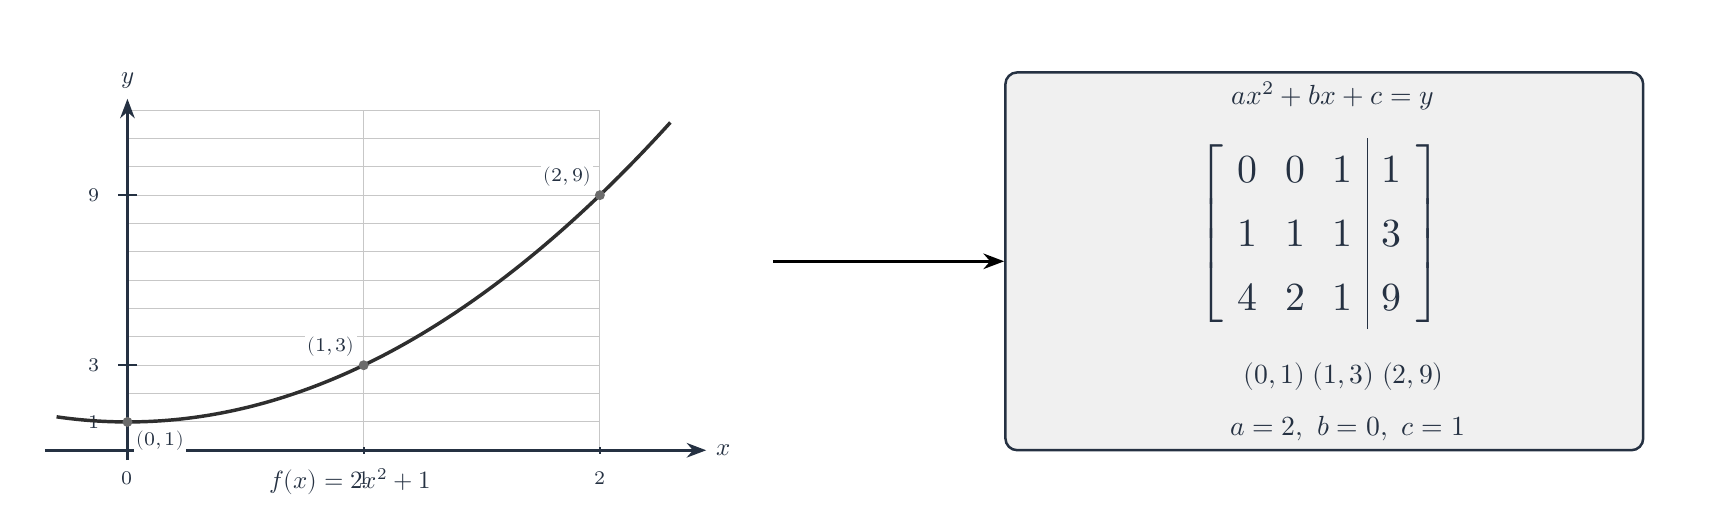
\begin{tikzpicture}[
  font=\sffamily,
  text=FigureInk,
  >={Stealth[length=3.4mm,width=2.4mm]},
  panel/.style={draw=FigureInk,line width=0.9pt,rounded corners=1.5mm,fill=PanelFill,
                minimum width=8.1cm,minimum height=4.35cm,align=center},
]
  \node[font=\bfseries\Large,align=center,text width=21cm] at (10.5,6.0)
    {插值把「曲線通過三個資料點」轉成係數的聯立方程組};

  \begin{scope}[shift={(1.15,0.75)},x=3cm,y=0.36cm]
    \draw[step=1,FigureGrid,line width=0.35pt] (0,0) grid (2,12);
    \draw[-{Stealth},FigureInk,line width=0.9pt] (-0.35,0) -- (2.45,0)
      node[right,font=\small] {$x$};
    \draw[-{Stealth},FigureInk,line width=0.9pt] (0,-0.35) -- (0,12.4)
      node[above,font=\small] {$y$};
    \foreach \x in {0,1,2}
      \draw[FigureInk,line width=0.6pt] (\x,0.12) -- (\x,-0.12)
        node[below=3pt,font=\scriptsize] {$\x$};
    \foreach \y in {1,3,9}
      \draw[FigureInk,line width=0.6pt] (0.04,\y) -- (-0.04,\y)
        node[left=3pt,font=\scriptsize] {$\y$};
    \draw[FigureCurve,line width=1.25pt,smooth,samples=121,domain=-0.30:2.30]
      plot (\x,{2*\x*\x+1});
    \foreach \x/\y/\placement in {0/1/below right,1/3/above left,2/9/above left}{
      \fill[FigurePoint] (\x,\y) circle[radius=1.8pt];
      \node[font=\scriptsize,\placement=3pt,fill=white,inner sep=1pt] at (\x,\y)
        {$(\x,\y)$};
    }
  \end{scope}
  \node[font=\bfseries\small] at (4.35,0.35) {$f(x)=2x^2+1$ 通過三個資料點};

  \node[panel] (system) at (16.35,3.15) {%
    \begin{minipage}{7.4cm}
      \centering
      \textbf{代入 $ax^2+bx+c=y$}\\[9pt]
      \Large$\FigureAugMatrix{0&0&1&1\\1&1&1&3\\4&2&1&9}$\normalsize\\[11pt]
      列分別對應 $(0,1)$、$(1,3)$、$(2,9)$\\[7pt]
      高斯消去得到 $a=2,\ b=0,\ c=1$
    \end{minipage}
  };
  \draw[-{Stealth},line width=1.0pt] (9.35,3.15) -- (system.west)
    node[midway,above,font=\small,align=center,fill=white,inner sep=2pt]
    {資料點提供\\三條方程式};
\end{tikzpicture}
\end{document}
